\specialsection{Введение}

Данное исследование является частью проекта по созданию централизованной системы управления потреблением энергии в зданиях общего назначения, тепловой и электрической. Одной из уникальных особенностей данной системы предполагается разработка и последующее применение интеллектуальных методов предсказания энергопотребления. Для предсказания энергопотребления надо понимать и уметь измерять те факторы, которые определяют необходимое количество электричества и тепла для здания в этот момент и в ближайшие несколько часов.

При постановке задачи регулирования для систем отопления, кондиционирования и вентиляции (ОВК), эксплуатирующие службы руководствуются двумя конкурирующими критериями: экономичностью работы системы и комфортностью внутренней среды. По различным оценкам, от 50 до 70 процентов всей расходуемой энергии приходится на ОВК. Таким образом, оптимизация потребления этого класса устройств, пусть даже на 5-10 процентов, повлечет за собой ощутимое снижение общего уровня расхода энергии. 

В основе данной работы лежит идея скомбинировать два основных подхода к моделированию микроклимата помещений: методы вычислительной термодинамики \cite{cfd}(CFD) и методы сетевых воздушных потоков (NAF). Точное решение задачи CFD на небольшом временном промежутке позволит смоделировать работу измерительного комплекса, оптимизировать вектор измеряемых величин, количество датчиков и их расположение в помещении. 


\newpage

\specialsection{Постановка задачи}

Основной вопрос - где в помещении расположить датчик температуры, который будет использоваться в составе централизованной системы эксплуатации здания, направленной на оптимизацию энергопотребления и обеспечение комфорта внутренней среды? Подобные системы используют методы управления с предсказывающими моделями. Поэтому предлагается критерий размещения датчика, учитывающий качество регресионных моделей, получаемых на основе показаний. 

Эта задача решается численными методами, так как сбор данных эмпирическим путем займет много времени и ресурсов. В стандартных офисных зданиях число отдельных зон может доходить до нескольких сотен, поэтому расстановка датчиков и считывание показаний очень трудоемкий процесс. В то же время, используя сгенерированную модель, мы можем определить значения на датчиках одновременно для всех интересующих расположений.

Для сокращения времени обследования здания, ускорения процесса развертывания сети, было предложено выделить в проекте два этапа - численное моделирование исследуемого помещения и анализ полученных данных.

На первом этапе будет смоделирован "Демонстрационный стенд Умного дома". Геометрия помещения задана в формате CAD. Моделирование будет производится в COMSOL Multyphysics \cite{comsol}. Целью является моделирование некоторого промежутка времени с хорошей точностью. Будет смоделирован процесс теплообмена внутри помещения и с окружающим воздухом, а также солнечная радиация. Значения внешней температуры будут взяты из собранного ранее датасета. Полученная модель будет использована далее.

На втором этапе будут выбраны точки возможного расположения датчика. Температуры в них будут импортированы в таблицу. Дальнейшая работа с полученными таблицами будет реализована на языке Python. Проанализировав потенциальные места расположения датчика методом, который предлагают в своей статье Пащенко А.Ф., Рассадин Ю.М. \cite{pashchenko-rassadin} (подробней об этом методе в главе \ref{algo-2}), сравнительным анализом найдем наилучшую точку размещения микроклиматического датчика. Для небольших помещений достаточно перебора потенциальных точек размещения, для больших помещений со сложной конфигурацией возможно применение градиентного метода поиска.


Результатом дипломного проекта станет отработанный метод построения упрощенной динамической модели характеристик воздуха в помещении, на основе которой может быть реализован последующий сбор реальных данных.

\newpage

\specialsection{Обзор предметной области}

Существуют два основных подхода моделирования микроклимата помещения \cite{ashrae}: метод вычислительной гидродинамики (CFD) и метод сетевых воздушных потоков (NAF). У каждого из этих подходов свои преимущества и недостатки.

Метод вычислительной гидродинамики может быть использован для моделирования помещения с микроскопической точностью. Динамика состояния помещения моделируется системой дифференциальных уравнений Навье-Стокса. Задаются геометрия помещения и граничные условия. В общем случае граничное условие определяет физическую задачу в определенных положениях. Часто физические явления осложняются одновременными тепловыми потоками (например, теплопроводностью через ограждение здания, получением тепла от обогреваемых внутренних объектов, солнечным излучением через остекление здания), фазовыми изменения (например, конденсация и испарение воды), химические реакции (например, горение) и механические перемещения (например, вентиляторы, перемещения жильцов).

Первым шагом в проведении CFD-анализа является разделение области на большое количество более мелких областей, называемых ячейками. Совокупность ячеек, составляющих область интереса, обычно называется сеткой или решеткой. Размер ячеек позволяет контролировать точность расчета.

CFD включает в себя решение связанных дифференциальных уравнений в частных производных, которые должны решаться одновременно или последовательно. Аналитических решений для моделирования внутренней среды не существует. Компьютерные численные процедуры являются единственным средством получения полных решений этих наборов уравнений.

Однако, высокая точность CFD компенсируется большими временными затратами как для аналитика при построении модели и интерпретации результатов, так и при решении компьютером смоделированных уравнений. Это ограничивает использование CFD для достаточно простых помещений и стационарных решений.

Существует достаточно много инструментов для моделирования, среди них: COMSOL Multyphysics \cite{comsol}, SimScale \cite{simscale}, EnergyPlus \cite{energyplus}, TRNSYS \cite{trnsys}

\newpage

В свою очередь, метод сетевых воздушных потоков может дать макроскопическое представление о здании путем решения системы уравнений сохранения массы и энергии. Сетевые модели воздушного потока идеализируют здание как совокупность зон, таких как комнаты, коридоры и места соединения воздуховодов, соединенных путями потока, представляющими двери, окна, вентиляторы, воздуховоды и т.д. Таким образом, пользователь собирает описание здания, соединяя зоны с помощью соответствующих путей потока. Сетевая модель прогнозирует потоки воздуха от зоны к зоне на основе характеристик давления и расхода в моделях путей и различий в давлении на путях. Три типа сил управляют потоком по путям: ветер, перепады температур (эффект стекания) и механические устройства, такие как вентилятор.

Как показано на рис. \ref{NAF}, модели сетей воздушного потока напоминают электрические сети. Поток воздуха соответствует электрическому току, при этом давление в зоне действует подобно напряжению в электрическом узле. Пути прохождения потока реагируют на резисторы и другие электрические элементы, включая активные элементы, такие как батареи (вентиляторы).

Весь этот процесс занимает гораздо меньше времени, что делает возможным моделирование всего здания, включая различные механические системы, в течение периода времени продолжительностью до года. Ограничения этого метода включают в себя гораздо менее детализированные результаты (например, отсутствие сведений о потоке воздуха внутри помещения). Отсутствие детализации в моделях зон сети делает CFD предпочтительным для прогнозирования теплового комфорта или проектирования систем вытесняющей вентиляции, где структура воздушного потока в помещении определяет интересующие величины.

Идея совместить эти два подхода была описана ранее в статье "Оптимизация HVAC-систем с помощью моделирования" \cite{blog}. Было смоделировано офисное помещение и находилось расположение датчика, который использовался для определения, в какой момент включать кондиционер. Тем не менее, авторы не ставили перед собой задачу придумать алгоритм, который позволит это делать для произвольной модели.

\begin{figure}[H]
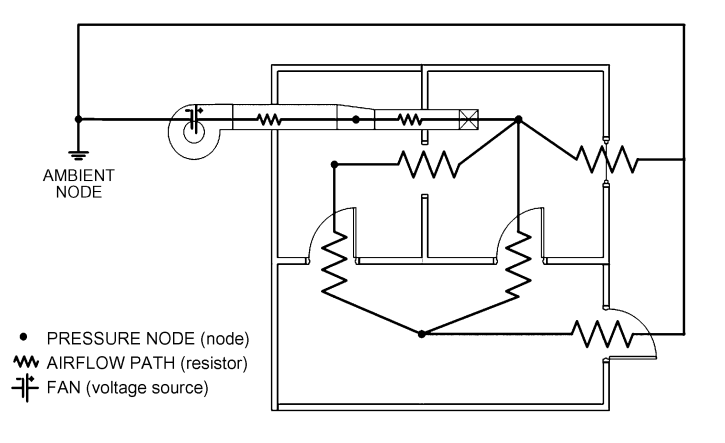
\includegraphics[width=\textwidth]{images/NAF_example.png}
\caption{}
\label{NAF}
\end{figure}

